\section{Sistema Solar}

En el observatorio CIAC se están planificando viajes turísticos por los distintos planetas del sistema solar, el único problema, es que se tienen muy pocos datos de los distintos astros almacenados en un archivo de texto \texttt{planetas.txt}. El formato de cada línea es \texttt{Nombre\#x;y;z} donde \texttt{x}, \texttt{y}, \texttt{z} son las posiciones de los planetas en un eje cartesiano de tres dimensiones.

\begin{figure}[h]
    \centering
    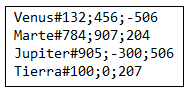
\includegraphics{Imagenes/planetas.png}
    \caption{\texttt{planetas.txt} }
\end{figure}

Se le pide a usted programar las siguientes funciones

\begin{itemize}
    \item[a.] \texttt{estaPlaneta(planeta,archivo)} que reciba un string con el nombre de un planeta y un archivo y retorne un booleano (True o False) dependiendo si el planeta está o no registrado en el archivo de texto.
    
    \begin{lstlisting}[style=consola]
>>> [*estaPlaneta('Jupiter','planetas.txt')*]
True
>>> [*estaPlaneta('Neptuno','planetas.txt')*]
False
    \end{lstlisting}
    
    \item[b.] \texttt{agregarPlaneta(planeta,archivo,coordenadas)} que reciba un string con el nombre del planeta a añadir, el nombre del archivo, y una lista con números enteros que representen las coordenadas del planeta. Esta función debe retornar True si se pudo añadir el planeta o False en caso contrario. Considere que un planeta no puede estar dos veces ingresado, ni puede ser reemplazado.
    
    \begin{lstlisting}[style=consola]
>>> [*agregarPlaneta('Neptuno','planetas.txt',[100,409,-708])*]
True
>>> [*agregarPlaneta('Jupiter','planetas.txt',[1001,4099,408])*]
False
    \end{lstlisting}
    
    \item[c.] \texttt{obtenerCoordenadas(planeta,archivo)} que reciba un string con el nombre del planeta y el el nombre del archivo y retorne una lista de enteros con las coordenas respectivas del planeta ingresado. Considere que siempre se ingresará un planeta presente en el archivo.
    
    \begin{lstlisting}[style=consola]
>>> [*obtenerCoordenadas('Tierra','planetas.txt')*]
[100, 0, 207]
    \end{lstlisting}
    
    \item[d.] \texttt{distanciaPlanetas(planeta1,planeta2,archivo)} que reciba como string el nombre de los planetas y archivo de texto y entregue la distancia directa entre ellos dos. Considere que la distancia entre dos puntos se calcula como $d=\sqrt{(x_1 - x_2)^2 + (y_1 - y_2)^2 + (z_1 - z_2)^2}$
    
    \begin{lstlisting}[style=consola]
>>> [*distanciaPlanetas('Tierra','Marte','planetas.txt')*]
1136.0079225075854
    \end{lstlisting}
    
\end{itemize}